% !TeX spellcheck = en_US
\documentclass[12pt]{article}
\usepackage[a4paper, margin=1.25in]{geometry}
\usepackage[utf8]{inputenc}
\usepackage{amsmath}
\usepackage{amsfonts}
\usepackage{amssymb}
\usepackage{graphicx}
\usepackage{mathtools}
\usepackage[hidelinks]{hyperref}  % most people dont know of this :3

\usepackage{float}
\usepackage{xfrac}

\usepackage{booktabs}
\usepackage{tabularx}

%\usepackage{subfig}
\usepackage{subcaption}
% \usepackage[margin=0.7in]{geometry}

\usepackage[backend=bibtex,style=verbose-ibid]{biblatex}
\addbibresource{citations.bib}

\usepackage{listings}
\usepackage{color}
\definecolor{dkgreen}{rgb}{0,0.6,0}
\definecolor{gray}{rgb}{0.5,0.5,0.5}
\definecolor{mauve}{rgb}{0.58,0,0.82}

\lstset{frame=tb,
  language=Python,
  aboveskip=3mm,
  belowskip=3mm,
  showstringspaces=false,
  columns=flexible,
  basicstyle={\small\ttfamily},
  numbers=none,
  numberstyle=\tiny\color{gray},
  keywordstyle=\color{blue},
  commentstyle=\color{dkgreen},
  stringstyle=\color{mauve},
  breaklines=true,
  breakatwhitespace=true,
  tabsize=3
}

\providecommand{\main}{..} 
\graphicspath{{\main/images/}{images/}}


\usepackage{pdfpages}

\usepackage[english]{babel}
\usepackage[autostyle, english = american]{csquotes}
\MakeOuterQuote{"}

\author{jcn514}
\title{IB Music Exploring Portfolio}
\date{\today}

\begin{document}
\maketitle
\tableofcontents

\pagebreak

\iffalse
heres an example of a code block
\begin{lstlisting}
        def intervalValues(z, n):
            return output $\sharp$ return the sequence of values
\end{lstlisting}

heres an example of an image
\begin{figure}[h]
\begin{center}
\includegraphics[scale=.37]{onefifteen} 
\caption{Sequences Generated by n = 1-15 on Argand Diagram}
\end{center}
\end{figure}
\fi

\section{Introduction}
I frequently encounter new styles, genres, techniques and theory that challenge my assumptions about music. Across a number of AOIs, I find myself pouring through musical scores, in combination with listening, sight-reading, and analyzing, trying to grasp at a genre’s conventions or motifs. One particular genre that piqued my interest was videogame music. To me, it’s fascinating how videogames leverage techniques from a deluge of genres, yet still conform to the technical or physical limitations of a game. For instance, a number of songs utilize only the square, sawtooth, and triangle tones due to the limitations of the original NES, making complex instrumentation or intricate polyphony impossible—instead opting for more jazz like qualities with melody-driven harmony.\autocite{collins_2007} Videogame composers manufacture memorable, impactful compositions that often can stand alone in their musical merit. This provoked me to explore how the jazz and videogame genres function for listening purposes (AOI 2) and to complement a game (AOI 3). I researched the intergenre connections among videogames music and the early foundations of jazz, discovering surprising connections along the way. To experiment with these fascinating ideas, I performed a cover of a Nintendo videogame classic in the style of ragtime and arranged an orchestral videogame song for a piano duet, falling under AOI 2 and 3 respectively.

\section{Experimenting as a Creator}

\subsection{Research 1: }



\section{Experimenting as a Performer}

\subsection{"Futile Devices" And My Foray into  Harp (AOI 1)}

In AOI 1, I chose to experiment with the song “Futile Devices” by Sufjan Stevens in the global context. This song is notable for its appearance in Call Me By Your Name, a 2017 movie exploring LGBTQ issues, serving as a form of political expression. With this, I chose to experiment with the Harp, an instrument with which I had absolutely no prior experience. I arranged, transposed and improvised on the main ostinato of the song, learning about the intricacies of the Harp to make this process more simple. I first familiarized myself with basic technique and the arrangement of the Harp’s pedals. From its tuning in $C$ with all pedals in the middle position, I tuned it to $C$ dorian by flattening the $3$rd and $7$th scale degrees. This was to make my life easier, transposing the harmony from $F\sharp$ dorian/$C\sharp m$ to $C$ dorian/$Gm$ so I could use the red and black strings to better orient myself (1 and 4 respectively). I began by playing the main arpeggio, outlining a $Cm7$/G, then transitioning to the $F7sus4$ and $F7$, using both hands to get it to tempo. In variation form, I progressively added more layers to the melody, eventually incorporating it in octaves in both hands. The last portion was the most challenging, where I played the second ostinato, outlining more chord extensions, in the RH, while maintaining both the first ostinato and the harmony in the LH. Overall, I was proud of my progress in about a week in-class and without any instruction.


\subsection{Reharmonizing a National Anthem (AOI 1)}

In AOI 1, I chose to experiment with the Russian Anthem, in the global context. I planned to experiment with the harmony of the piece—specifically by reharmonizing elements of it and varying the key. I planned to do this because it employs a simple harmony with virtually no chord extensions or modulations. By experimenting with it, I will convert it towards a more jazz-influenced style, with a more complicated harmony, including a number of distant modulations scattered throughout. In this way, I plan to transform the melody into a different context, enriching its simplicity with new harmony. 

\begin{figure}[ht]
\centering
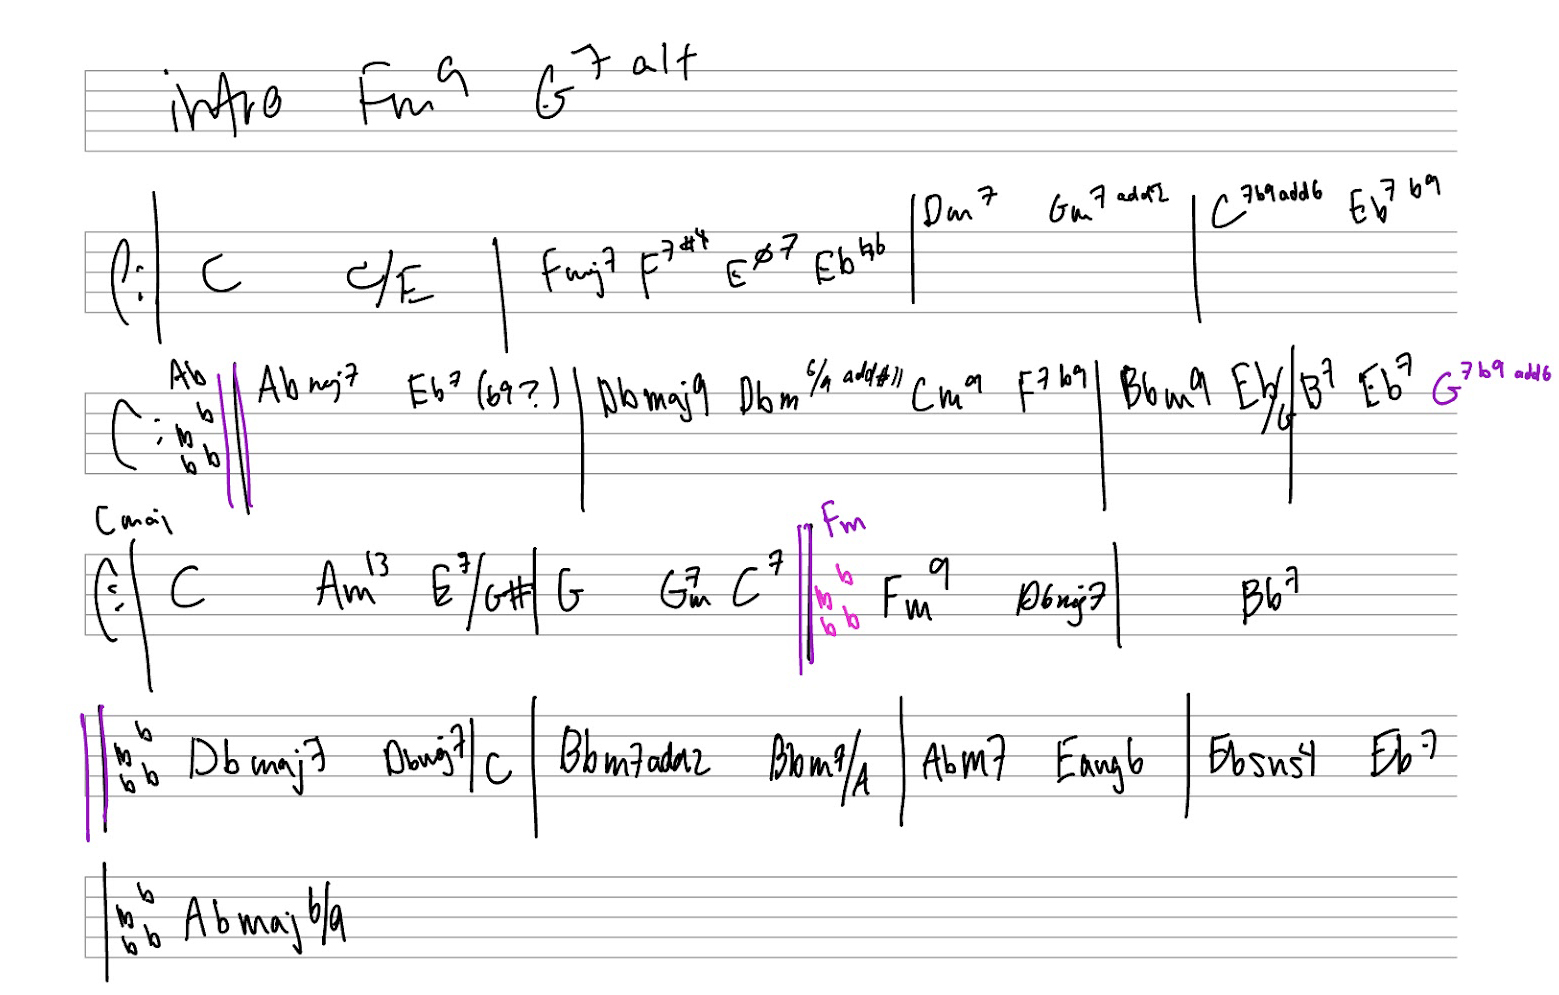
\includegraphics[width=0.85\linewidth]{anthem}
\caption{My Handwritten Lead Sheet for the Russian Anthem Reharm}
\label{fig:anthem}
\end{figure}

\subsection{Experimenting with Coltrane's "Alabama" Vamp (AOI 1)}

In AOI 1, I am choosing to experiment with John Coltrane’s “Alabama,” in the local context. This song is AOI 1, because Coltrane intended it to reflect the state of the civil rights movement in the US. It’s said that he attempted to mimic the cadences of Martin Luther King Junior’s speeches with his improvisational melody. I plan to experiment with the idea of sitting on a single harmony with improvisation in the melody. In Coltrane’s work, he sits on this C minor harmony, with a melodic emphasis on a $\flat7–1$ resolution, or a $v–i$ resolution. I will experiment with a $Fm–F$ dorian harmony in an improvisational way, focusing on the sound of a $iv–i$ resolution, to create a similar tone to Coltrane in a novel way.

    
\section{Exploring as a Creator Written Statement}

To explore unfamiliar territory as an arranger, I chose to reinvent an orchestral piece for four-hands piano. My stimulus was “Main Theme” from Octopath Traveler, composed by Yasonuri Nishiki. I came across this song within a videogame I had not played. I was intrigued by the instrumentation and western style despite its Japanese origin. I hadn’t written for four hands on the piano; I was excited to undertake the challenge. Therefore, this project falls under Global Context and AOI 3, since I adapted music to an unfamiliar instrumentation and the music evokes emotion within the game. 

My initial brainstorm consisted of exploring unfamiliar music in a variety of genres. I decided on four-hands piano after listening to works in these styles by Schubert and Brahms, notably Schubert’s "Sonata in C major for piano four-hands, D 812", wherein he uses block chords and intertwines melody between the primo and secondo players. Much of this research informed techniques I used in my arrangement. For instance, I didn't restrict my melody to only the top voice; at times I had a pianissimo \textit{sans acentuacion} ostinato in the top voice adding glitter to the harmony. Additionally, I incorporated the technique of a call/response melody in the treble of the secondo piano. Overall, I found my research useful in expanding my musical vocabulary within this style.

My 32-bar composition derives from the first section of the orchestral piece. Using piano dynamics, I tried to emulate the chugging chords in the strings section. In the first section, I also used \textit{acciaccatura} to emulate the sound of the wind section. I often deviated from the stimulus piece by adding in extra chord extensions and voicing the melody in 3rds 5ths and 6ths to capture the orchestra's thick texture. After the sudden key change, I employed dynamic contrast between the secondo piano playing melody and the primo piano contributing to harmony with ostinato trill-like chords using various diatonic 2nds in the appropriate mode (e.g., $A\flat$ Lydian, $E\flat$ Dorian, etc.). Lastly, I incorporated syncopation and thick cluster-chords to give the final two sections momentum and emphasis.

Overall, I was pleased with the outcome of my exploration, although I anticipated it would be less difficult to do. The most time-consuming part was adapting the technique such that both pianists could play notes comfortably without awkward overlap. This forced me to interchange my melodies between hands and to employ, at times, complex fingerings. If I were to complete this assignment once more, I would record each part since the sampled piano on the notation software made certain parts sound muddy and hampered the dynamic contrast.


\section{Exploring as a Performer Written Statement}

For the task of Exploring as a Performer, I chose the “World Ending Theme” from Nintendo's Super Mario World. This song falls under local context and the AOI 2. Although I'd never played Super Mario world, this song has a local context because I've listened to this piece for enjoyment. Furthermore, this piece falls into AOI 2 because I adapted this song to a rag-time genre, which is a performance-based convention. 
My initial brainstorming ideas included emphasizing the rag-time-like sound with a jumping left-hand and an accentuation of the swing rhythm. I focused on maintaining the general structure and feel of the harmony throughout; the changes I made were in voicing chord extensions and voice-leading. With these ideas in mind, I researched rag-time conventions. And, after deep-diving into the conventions of Joplin, I felt I had a strong foundation. I tried to implement techniques including emphasis on a dominant-tonic bass on strong beats and block chords on weak beats to create the syncopated swing melody. I also focused on the crossrelation between the $\flat 3$rds and $\natural 3$rds and the use of altered dominants, like the augmented dominant $7$th.
 
For the first week, I explicitly wrote out the melody to better understand the swing rhythm. I then practiced the muscle memory for the jumps in the left-hand. Despite my piano background, I had limited experience with these left-hand figures. This took time because I intentionally challenged myself with wide LH intervals, voicing the strong beats in octaves and the chords on weak beats with a mix of inverted three- and four-note chords, and I found it initially difficult to play the RH and LH together. Another idea I developed while practicing was to tighten the voice leading by altering the chord extensions. For example, in the ending $\Rn{2}–\RN{5}–\Rn{1}$ cadence, I complexified the chords with an $Fmaj6$ over $D$ (outlining a $Dm9$), then a $F7(\flat 5)$ over $G$ (a $Galt$), and resolving to a $Cmaj\sfrac{6}{9}$. Here, the upper voice walks two semitones from $E$ to $D$ grounding this cadence. 
 
As I progressed, the song became easier and more enjoyable to play. Recording the performance was not exceedingly difficult; it only took around five takes. It also took a slight amount of work to set up the stereo microphone setup and to tweak my adjustments to the sound. Overall, from this project I was proud to see that my piano abilities could adapt to novel styles and situations, despite my inexperience.

\section{References}
\printbibliography[heading=none]

\section{Appendix}


\begin{table}[H]
\centering
\begin{tabularx}{0.9\textwidth}{@{}lX@{}}
\toprule
\textbf{Track}                                            & \textbf{Timestamp}                                                  \\ \midrule
Country Club Rag – Scott Joplin                  & 0:00                                                                \\[4pt]
Piano Concerto for the Left Hand – Maurice Ravel & \begin{tabular}[c]{@{}l@{}}PART 1: 0:41\\ PART 2: 1:05\end{tabular} \\[10pt]
Rude Buster – Toby Fox                           & 1:42                                                                \\[5pt]
Wii Shop Theme – Nintendo                        & 2:17                                                                \\ \bottomrule
\end{tabularx}
\caption{Audio tracks for Music Research}
\vspace*{1cm}
\centering
\begin{tabularx}{0.8\textwidth}{@{}lX@{}}
\toprule
\textbf{Track}                   & \textbf{Timestamp} \\ \midrule
Exploring as a Creator           & 0:00               \\
Ending Theme – Super Mario World & 1:13               \\
Exploring as a Performer         & 1:58               \\ \bottomrule     
\end{tabularx}
\caption{Audio evidence for Exploring as a Creator/Performer}
\end{table}

\pagebreak

\begin{figure}[H]
\centering
\begin{tabular}{cc}
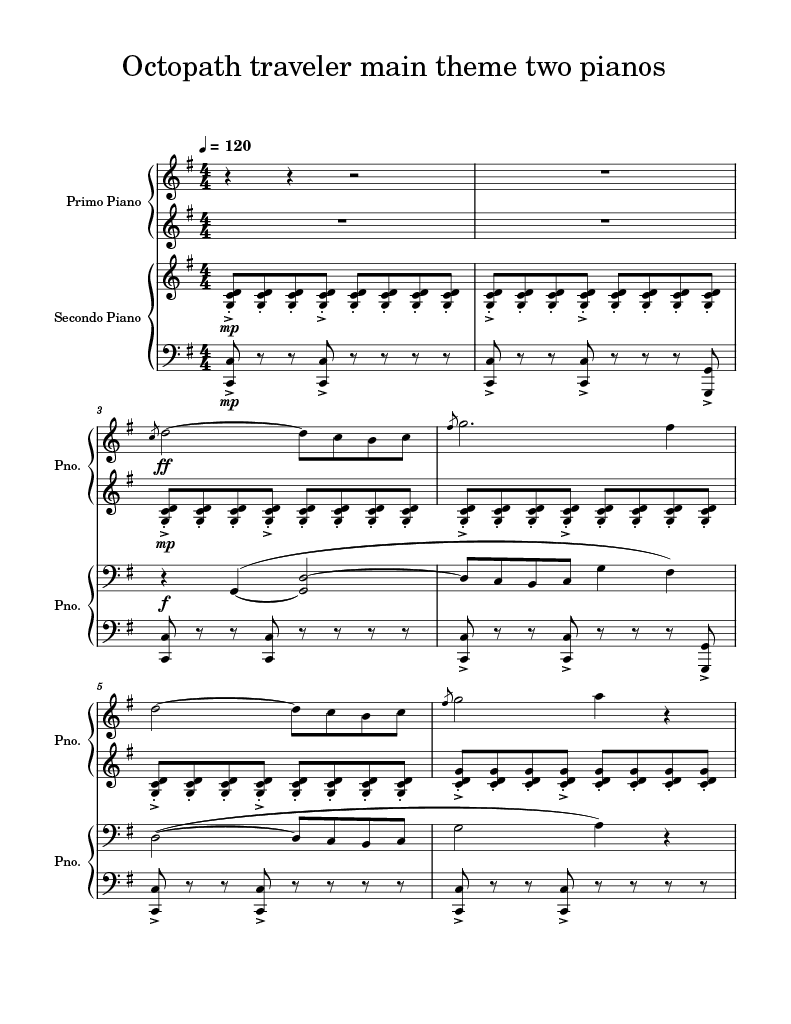
\includegraphics[width=.4\linewidth, trim=30 100 30 20, clip]{octopathscore/octopathscore1024_1.png} &
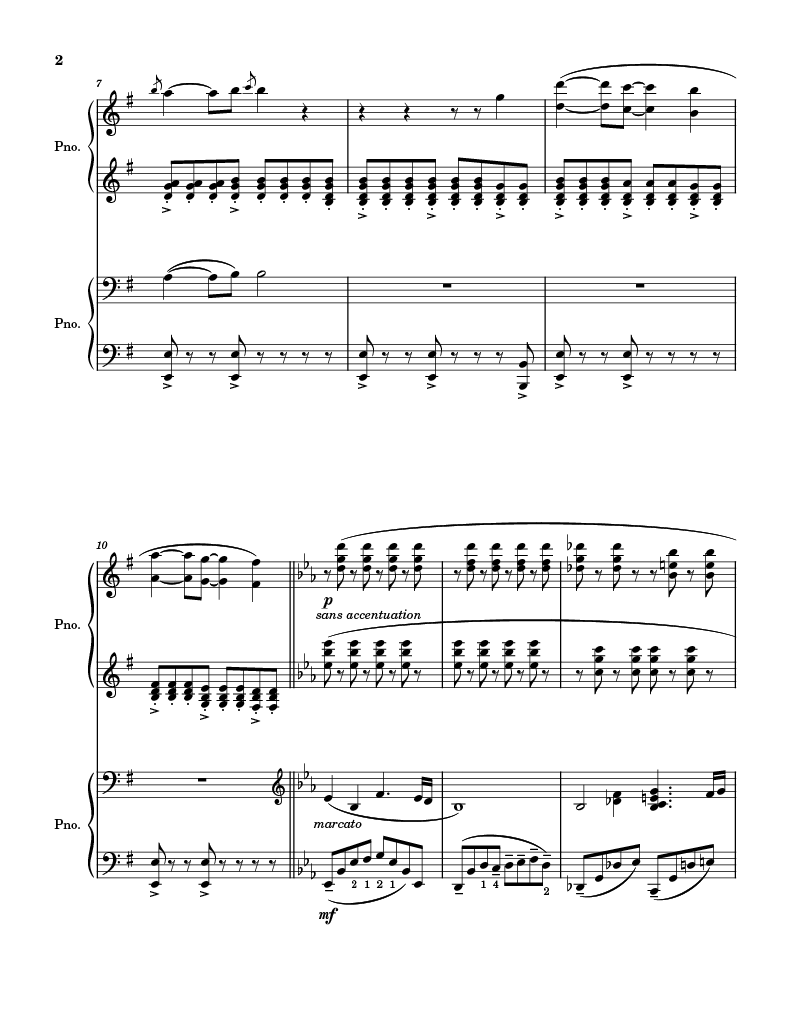
\includegraphics[width=0.4\linewidth, trim=30 100 30 20, clip]{octopathscore/octopathscore1024_2.png} \\
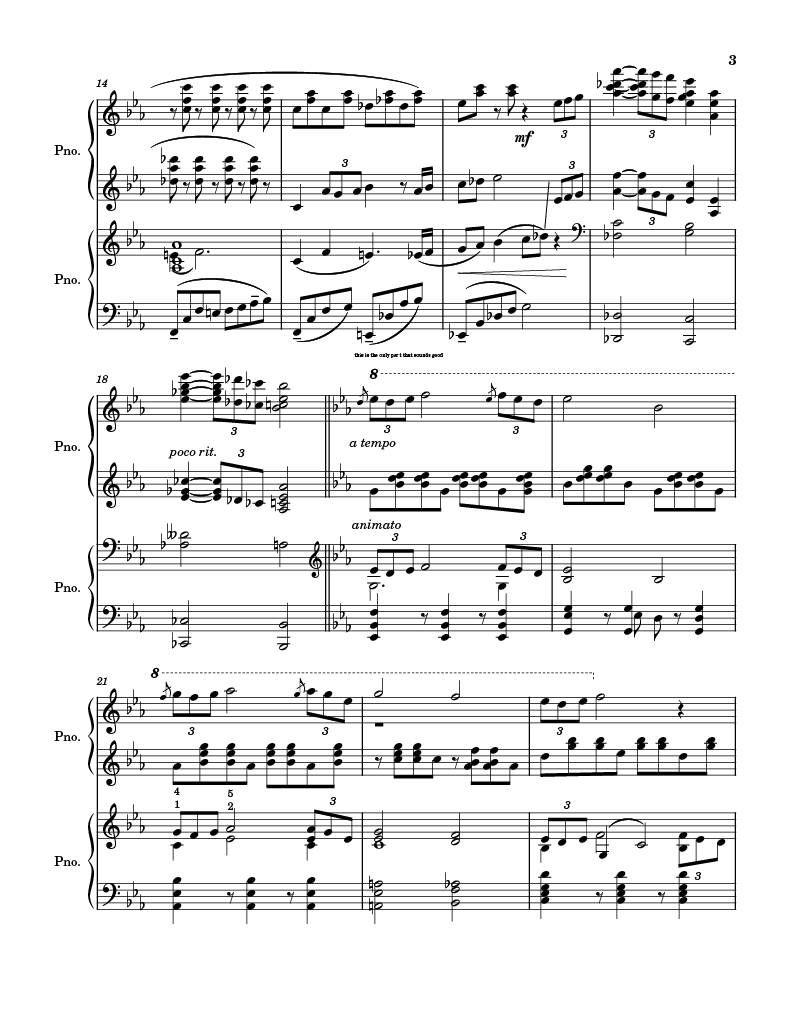
\includegraphics[width=0.4\linewidth, trim=30 100 30 20, clip]{octopathscore/octopathscore1024_3.png} &
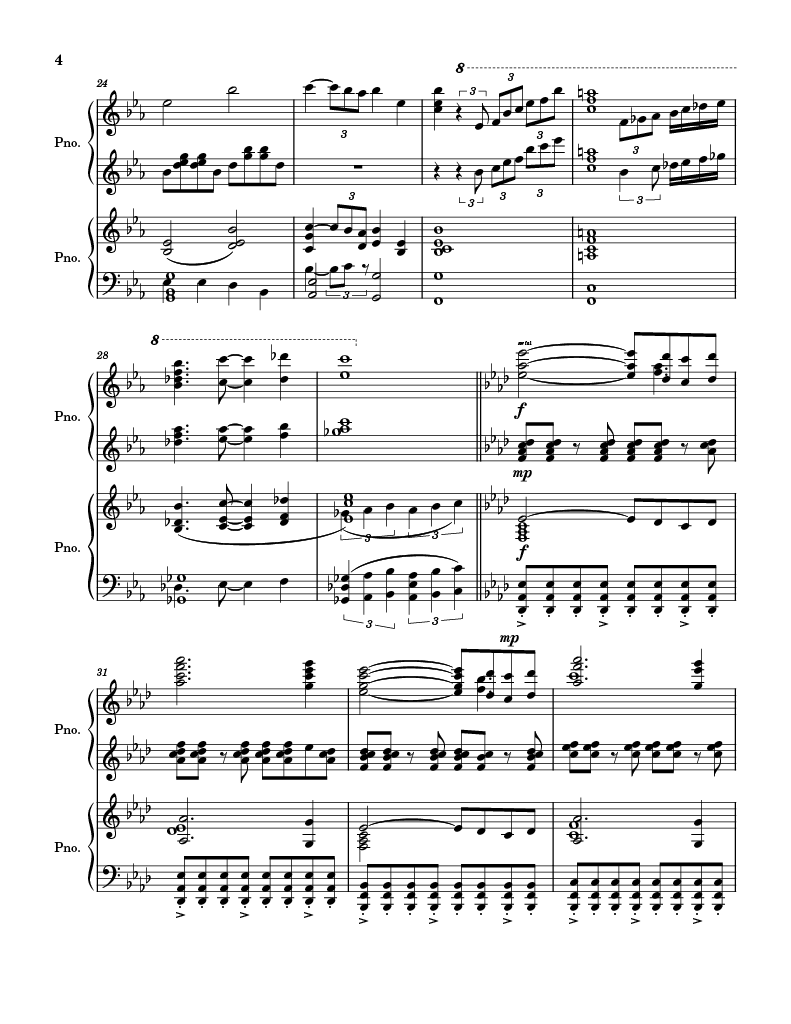
\includegraphics[width=0.4\linewidth, trim=30 100 30 20, clip]{octopathscore/octopathscore1024_4.png}
\end{tabular}
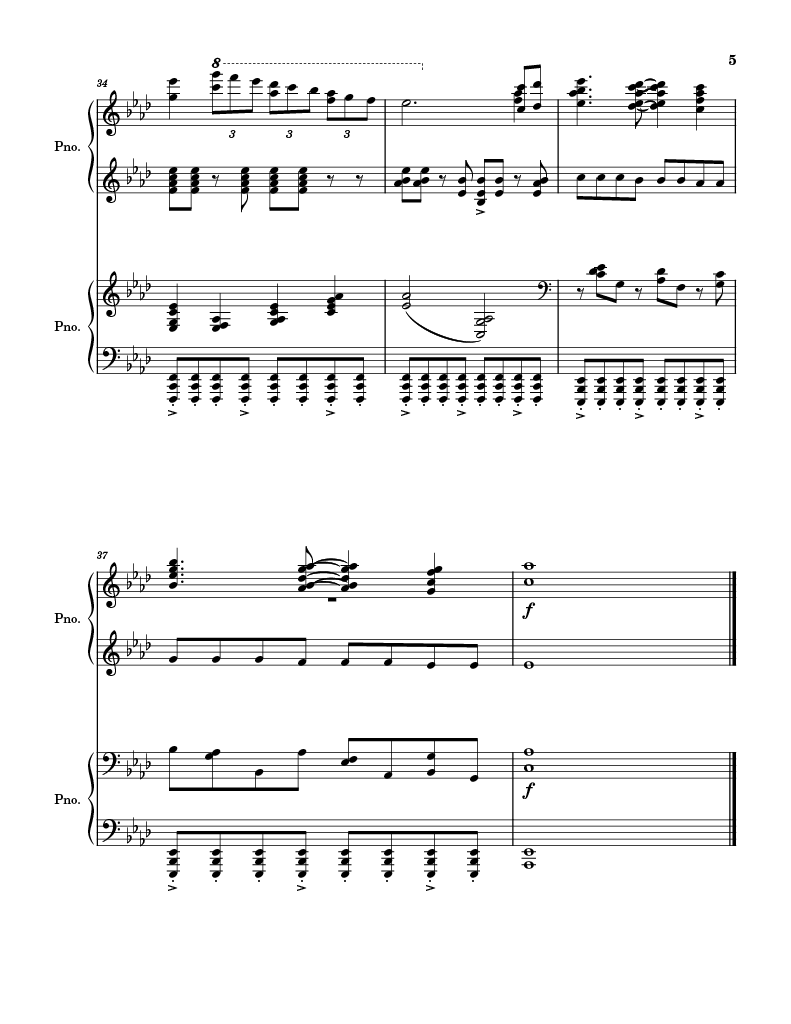
\includegraphics[width=0.4\linewidth, trim=30 100 30 20, clip]{octopathscore/octopathscore1024_5.png}
\caption{My Arrangement Score for Exploring as a Creator}
\end{figure}




\end{document}